\section{Tax Incentives \& Family Transfers: Proposition 19}\label{sec:prop19}

\subsection{Institutional background}

Proposition~13 (1978) fixed each California parcel's assessed value at its
acquisition price, with growth capped at two percent per year; reassessment
to market value occurs only at a change in ownership. Proposition~58 (1986)
exempted parent-to-child transfers from this reassessment---for a principal
residence of unlimited value plus up to \$1 million of assessed value of
other property---and Proposition~193 (1996) extended the exemption to
grandparent-grandchild transfers. A child could therefore inherit not just a
house but its decades-old tax bill, and keep that tax bill while renting the
house out. The Legislative Analyst's Office estimated that 60,000 to 80,000
inherited properties escaped reassessment each year under this regime
\citep{lao2017inheritance}.

Proposition~19, passed by voters on November 3, 2020, narrowed the exclusion
sharply, effective February 16, 2021: it now applies only when the home was
the parent's principal residence \emph{and} the child makes it their own
principal residence within a year, and only up to the inherited taxable value
plus \$1 million (inflation-adjusted); the exclusion for rentals, vacation
homes, and other non-primary-residence property was eliminated, with a
carve-out for family farms \citep{boe2025prop19, lao2020prop19}. For an otherwise eligible non-occupant heir, the reform removes the inherited-assessment advantage. This raises the tax cost of retention relative to sale, although the family may respond by changing paperwork, timing, occupancy, or ownership rather than by listing the home.
County assessors reported a flood of parent-child filings ahead of the
deadline.\footnote{Sonoma County, for example, received roughly five times
its typical volume of parent-child exclusion filings in the weeks before the
February 15, 2021 deadline (North Bay Business Journal, February 2021); the
Los Angeles County assessor accumulated a multi-year backlog of roughly
20,000 claims (Los Angeles County Auditor-Controller, 2025).} The reform's
other arm---expanded portability of assessments for movers aged 55 and over,
effective April 1, 2021---affects market sales rather than family transfers;
the market-sale placebo therefore need not be an untreated control. We report its adjustment separately from the synthetic-control estimates.

Throughout this section, ``family transfers'' means the broad class
(same-surname, cross-surname, and estate/executor deeds), measured monthly by
state from the event panel; results including trust self-transfers are
reported as robustness.

\subsection{Retiming: the rush to beat the deadline}

Figure~\ref{fig:bunching} plots monthly California family transfers against a
transparent counterfactual: California's 2019 volume in the same calendar
month, scaled by contemporaneous family-transfer growth in the other 49 states and DC. The counterfactual thus inherits both California's seasonality
and national shocks---COVID disruption, the 2020--2021 housing boom, the
estate-planning surge---while excluding California from the donor pool. Before
passage, it fits tightly: over 2018m1--2020m10, the mean absolute monthly error
is 3.9 percent and the RMSPE is 5.7 percent.

\begin{figure}[!t]
  \centering
  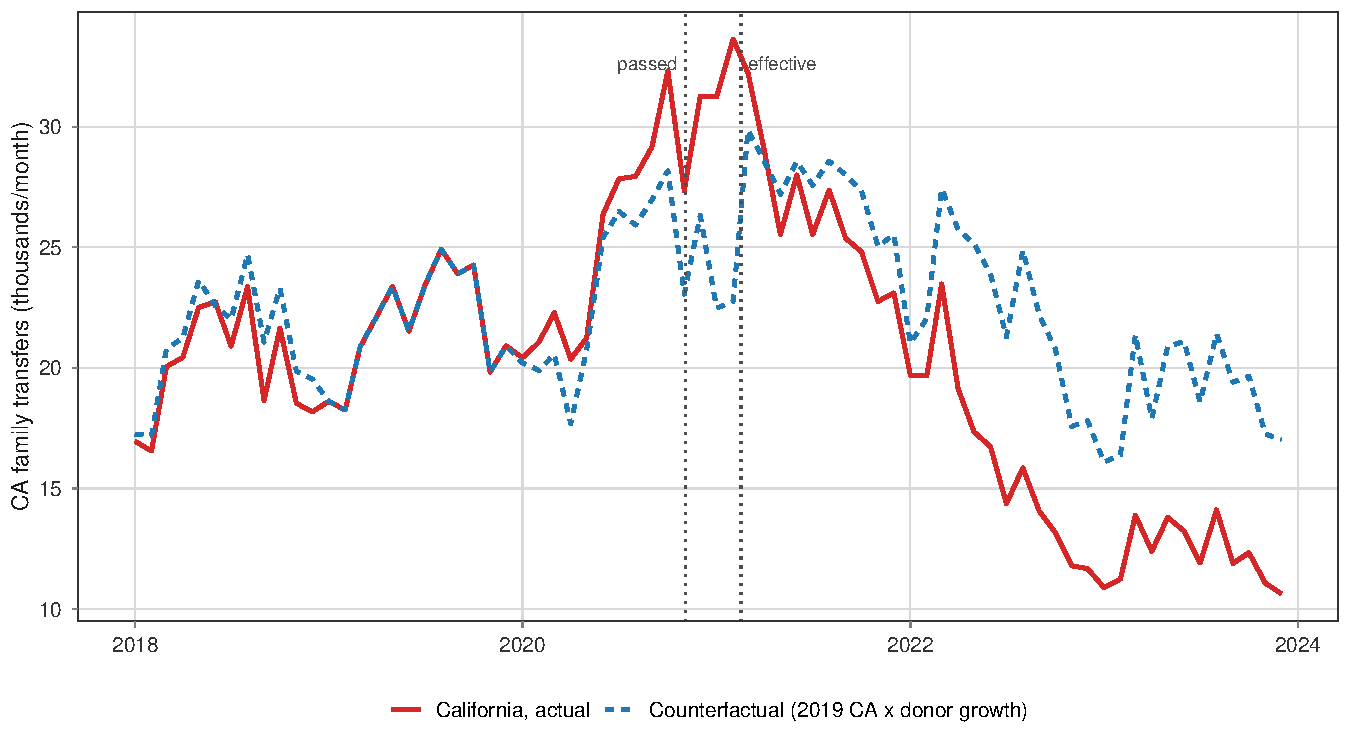
\includegraphics[width=0.92\linewidth]{figures/F4_prop19_bunching.pdf}
  \caption{California monthly family transfers (broad class) versus
  counterfactual (CA 2019 same-calendar-month volume $\times$ donor-state
  growth). Dotted lines: November 3, 2020 (passage) and February 16, 2021
  (parent-child provisions effective).}
  \label{fig:bunching}
\end{figure}

California tracks the counterfactual closely until November 2020. Between
passage and the deadline, the two series tear apart: from November 2020
through February 2021, actual family transfers total 123,486 against a
counterfactual of 94,615---an excess of 28,871 deeds, 31 percent above
counterfactual, crammed into four months. February 2021, ordinarily the
year's quietest month, became the busiest family-transfer month in the
2018--2023 California series. This is the anticipatory bunching that notch
designs recover for taxed market transactions \citep{bestkleven2018notches,
slemrodwebershan2017dc}, reproduced in transfers with no price: families
re-timed successions to bequeath a tax basis. In leave-one-out placebo
counterfactuals, California's anticipation gap is third of fifty-one in raw
size ($p=0.059$) but first after dividing each state's gap by its own
pre-period RMSPE ($p=0.020$). The concentration around the deadline supports a tax-timing interpretation, although monthly counts do not identify the exact legal transfer date or rule out every contemporaneous influence.

\subsection{The steady-state decline}

Retiming alone would imply a transitory post-deadline trough followed by
recovery. Instead, the gap persists and widens. From March 2021 through
December 2022, actual transfers run 85,351 below counterfactual (16
percent); by 2023, California family transfers (147,441) are 41 percent below
their 2018--2019 average (251,256)---while national volumes returned to
trend. A donor-weighted synthetic control sharpens the comparison. Following
\citet{abadie2010synthetic}, we build a synthetic California from a convex
combination of the other 49 states and the District of Columbia, with
weights chosen to match California's pre-reform family-transfer trajectory.
Because California is the largest state---an outlier in the \emph{level} of
transfers, which forces a level-matched synthetic onto a single large donor---we
match on each state's volume normalized to its own 2018--2019 mean. The
synthetic reproduces California's pre-reform path to a root mean squared error
of 5.0 percent (Figure~\ref{fig:scm}); after the February 2021 deadline,
California's family transfers run 33 percent below synthetic California through
2022--2023, and the gap lies at the extreme lower edge of the donor placebo
distribution (Figure~\ref{fig:scm_envelope}).

\begin{figure}[!t]
  \centering
  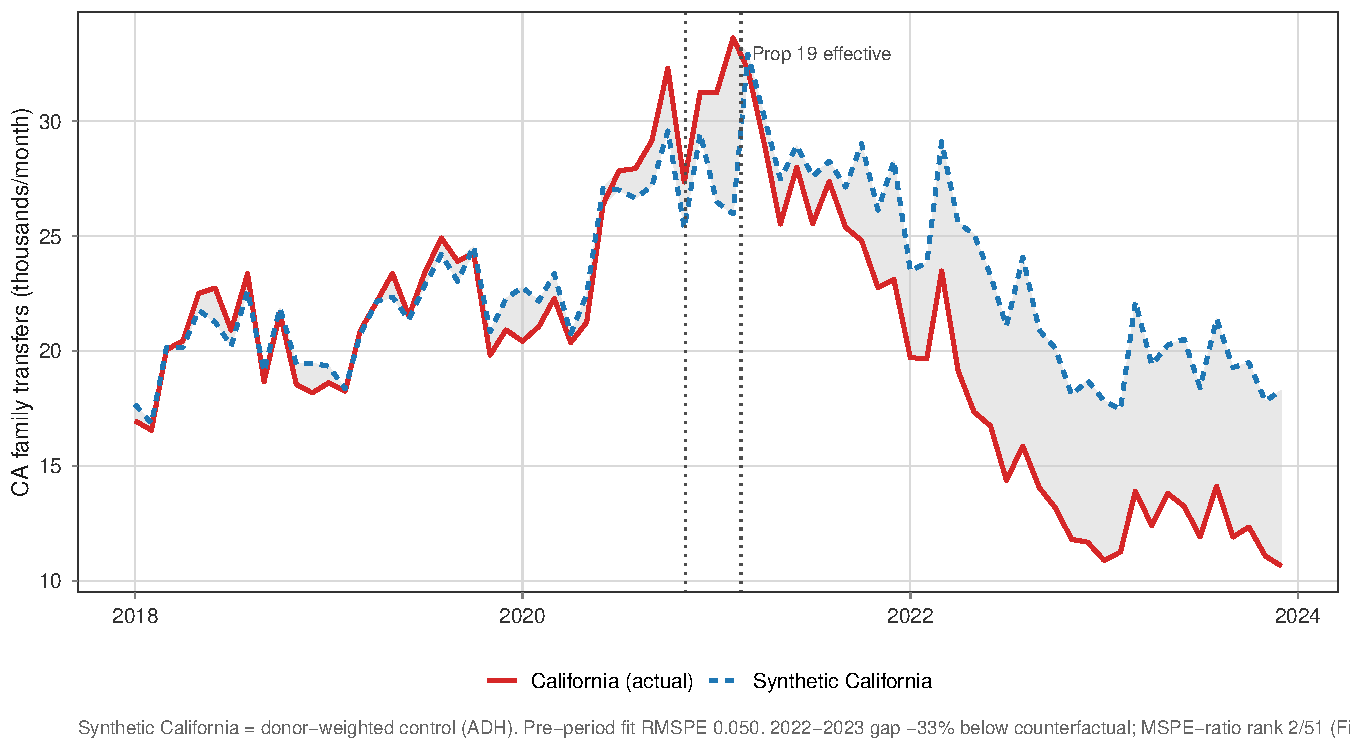
\includegraphics[width=0.9\linewidth]{figures/F5_scm_california.pdf}
  \caption{California monthly family transfers against a donor-weighted
  synthetic California \citep[normalized-index match;][]{abadie2010synthetic}.
  The series track closely before the reform and diverge after the deadline.
  Dotted lines: passage (November 3, 2020) and the parent-child effective date
  (February 16, 2021).}
  \label{fig:scm}
\end{figure}

\begin{figure}[!t]
  \centering
  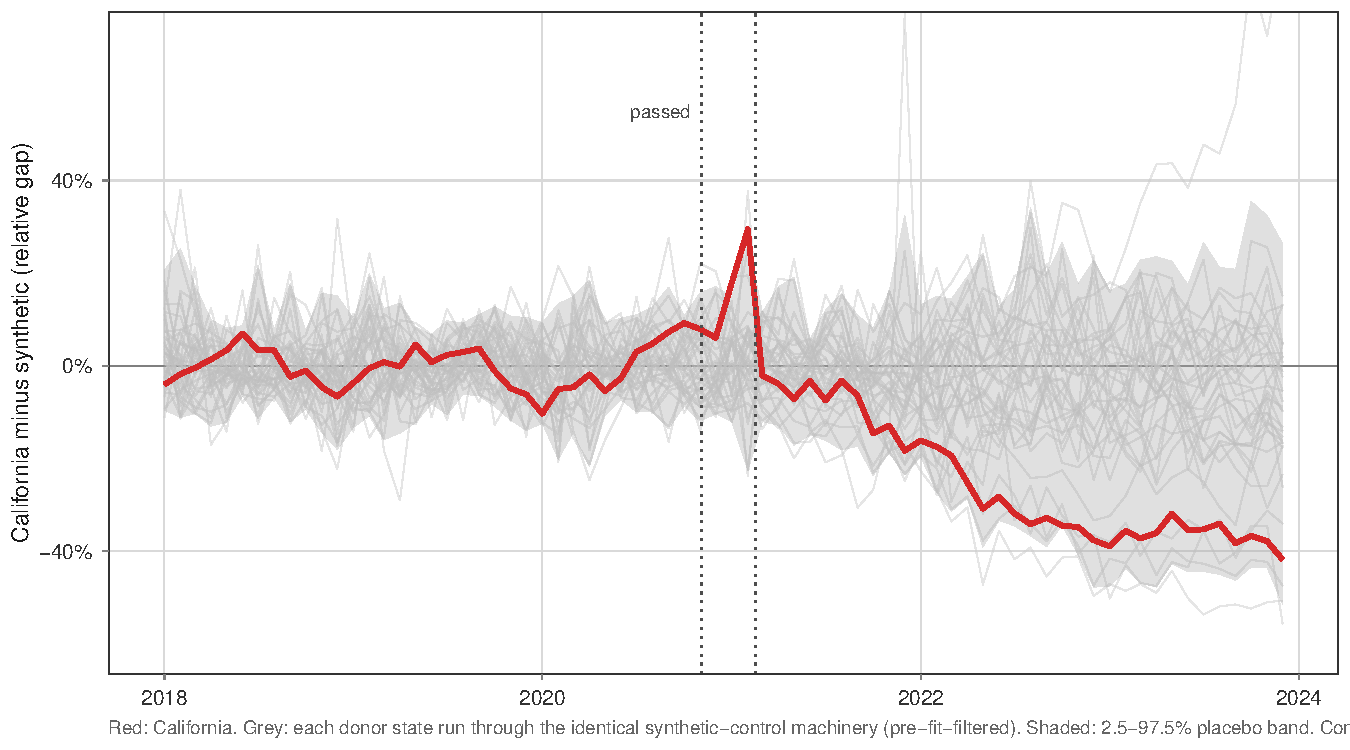
\includegraphics[width=0.9\linewidth]{figures/F6_scm_gap_envelope.pdf}
  \caption{California's relative gap from synthetic control (red) against the
  same gap computed for each donor state run as a placebo (grey lines), with a
  shaded 2.5--97.5 percentile band over donors that fit California comparably
  well before the reform. California lies at the extreme lower edge across
  2022--2023.}
  \label{fig:scm_envelope}
\end{figure}

The difference-in-differences estimates in Table~\ref{tab:prop19} formalize
this. Using state-by-year counts for 2017--2019 versus 2022--2023 (the
transition years 2020--2021 are excluded as contaminated by anticipation and
retiming), with state and year fixed effects, log family transfers fall by
0.425 (s.e.\ 0.035) in California relative to other states---35 percent. The
placebo column shows log market sales falling 0.163 (15 percent) over the
same window, California's general post-rate-shock slump; netting it out
leaves a 23 percent decline specific to family transfers, roughly 58,000
transfers per year against the 2018--2019 base. Reclassification into trusts
cannot explain it: including trust self-transfers in the family aggregate
yields a decline of 0.241 log points (21 percent).

Two pieces of evidence address the design's limitations. First, because
California is a single treated unit, we use the synthetic-control in-space
placebo: each donor state is assigned the treatment in turn, and the ratio of
its post- to pre-reform mean squared prediction error measures how extreme its
post-period deviation is relative to its own pre-reform fit. California's ratio
is the second largest of fifty-one units, including DC---a placebo-rank $p=0.039$
(Appendix Figure~\ref{fig:scm_mspe})---using a different statistic from the transparent counterfactual's rank-based inference
\citep{conley2011inference}. A demographic adjustment changes the estimated magnitude: re-estimating the synthetic control on family
transfers per resident aged 65 and over (American Community Survey one-year
estimates) leaves a 27 percent gap ($p=0.137$). These specifications use different denominators and identifying assumptions. The 27--33 percent range summarizes sensitivity across them; it is neither a confidence interval nor an identified lower and upper bound. For the market-adjusted DiD, the state-placebo $p$-value is 0.176. The SCM Conley--Taber-style interval also includes zero (Appendix~\ref{app:robustness}). The welfare exercise in Section~\ref{sec:welfare} retains this uncertainty rather than treating the response as precisely known.

Second, timing. A monthly event study resolves what the annual specification
hides. We regress $\log$ family transfers on California-by-month indicators
with state and year-month fixed effects, the other 49 states and DC as
controls, and the 2018--2019 months pooled as the omitted baseline.
Figure~\ref{fig:event_study} traces the whole path: California sits near its
2018--2019 baseline in early 2020, drifts upward through the anticipation period
as Proposition~19 reaches the ballot and passes, spikes to $+0.32$ log points in
February 2021---the deadline month---and then settles into a persistent decline
of $0.3$ to $0.5$ log points through 2022--2023. An annual event study reports
essentially zero for 2021 only because the pre-deadline rush and the
post-deadline collapse cancel within the calendar year; at monthly resolution
the two are plainly distinct, and the post-reform level shift is unmistakable.
The missing annual flow, roughly \WelfareFlow\ deeds, is of a similar order
to the Legislative Analyst's 60,000--80,000 count of tax-excluded inherited
properties per year. The two quantities cover different populations and
units; this comparison does not validate the estimated deed response or
identify how many properties change allocation.

\begin{figure}[!t]
  \centering
  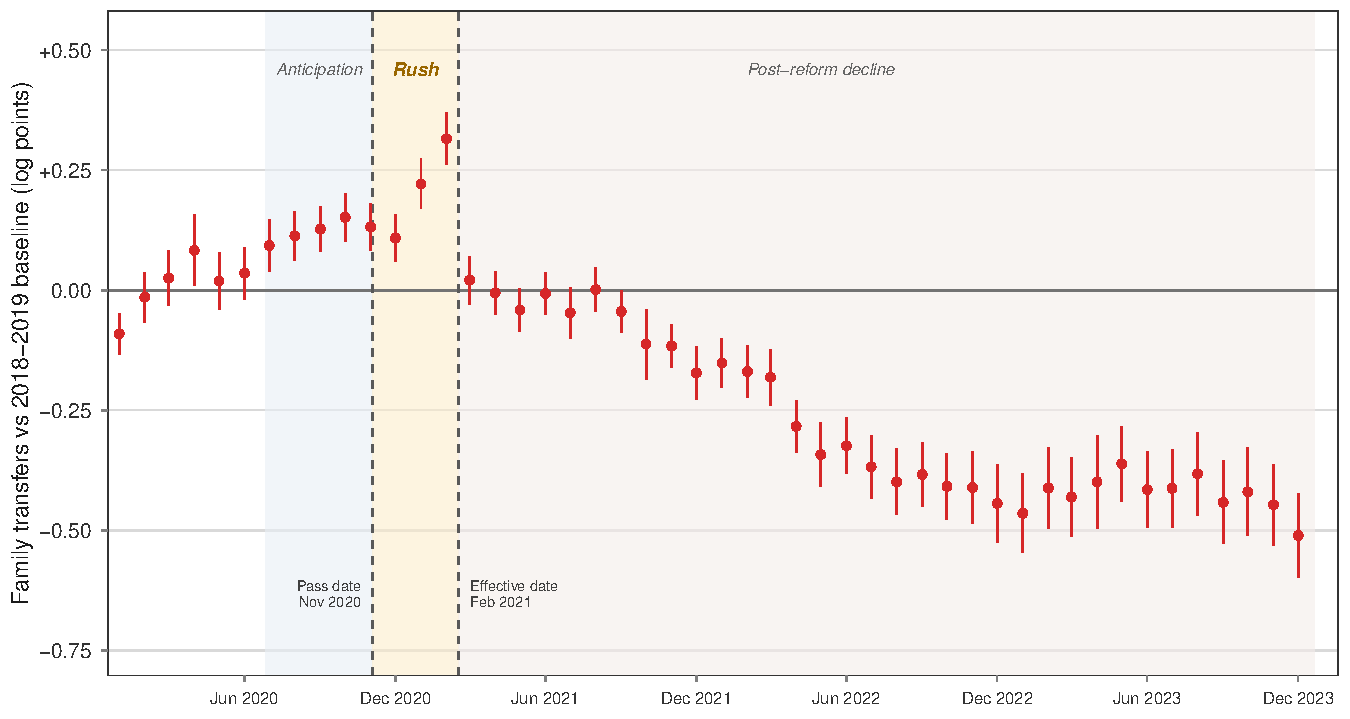
\includegraphics[width=0.95\linewidth]{figures/F_event_study_monthly.pdf}
  \caption{Monthly event study of California family transfers. Points are
  California-by-month coefficients from a regression of $\log$ family transfers
  on state and year-month fixed effects, with the 2018--2019 months pooled as
  the omitted baseline and the other 49 states and DC as controls. Whiskers
  are 95 percent state-clustered confidence intervals. Shaded regions mark the
  anticipation build-up (ballot to passage), the rush between passage and the
  February 16, 2021 effective date, and the post-reform period; dashed lines
  mark the passage and effective dates.}
  \label{fig:event_study}
\end{figure}


\begin{table}[htbp]
   \caption{\label{tab:prop19} Proposition 19: volume, selection, and composition}
   \centering
   \scriptsize
   \begin{tabular}{lccccc}
      \tabularnewline \midrule \midrule
      Dependent Variables: & log(n\_fam) & log(n\_market) & \multicolumn{2}{c}{Sold within 24m} & Absentee share\\
      Model:                     & (1)            & (2)             & (3)      & (4)      & (5)\\  
      \midrule
      \emph{Variables}\\
      CA $\times$ Post           & -0.4253        & -0.1626         & -0.0178  & -0.0104  & -0.0017\\   
                                 & (0.0352)       & (0.0293)        & (0.0032) & (0.0019) & (0.0032)\\   
      Ann. placebo rank          & 5/51 (p=0.098) & 17/51 (p=0.333) &          &          & \\  
      Fam. $-$ market log effect & -0.263         &                 &          &          & \\  
      Monthly pre-fit rank       & 1/51 (p=0.020) &                 &          &          & \\  
      \midrule
      \emph{Fixed-effects}\\
      State                      & Yes            & Yes             & Yes      & Yes      & Yes\\  
      Year                       & Yes            & Yes             &          &          & \\  
      Cohort month               &                &                 & Yes      & Yes      & Yes\\  
      \midrule
      \emph{Fit statistics}\\
      Observations               & 255            & 255             & 1,836    & 1,836    & 1,836\\  
      R$^2$                      & 0.98575        & 0.98961         & 0.84935  & 0.85148  & 0.90779\\  
      \midrule \midrule
      \multicolumn{6}{l}{\emph{Clustered (State) standard-errors in parentheses}}\\
   \end{tabular}
   
   \par \raggedright 
   Cols (1)-(2): state-year counts, 2017-2019 vs 2022-2023. Cols (3)-(5): cohort cells (2017m1-2018m12 vs 2021m7-2022m6), weighted by cell size. Clustered (state) SEs are shown only for scale; single-treated-state inference uses placebo ranks. The monthly pre-fit rank is the 2022-2023 California gap divided by its 2018m1-2020m10 counterfactual RMSPE, ranked against leave-one-out placebo states.
\end{table}




\subsection{Selection: who still keeps the house}

If the reform discourages transfers to heirs who would otherwise retain the house for its tax basis, the surviving transfers can become more selected toward long-term retention. This is a possible mechanism, formalized in Section~\ref{sec:framework}, rather than an implication of the volume estimate alone.
We take
family-transfer cohorts from two clean windows---January 2017 to December
2018 (pre) and July 2021 to June 2022 (post, after the retiming
turbulence)---and measure whether each transferred home reaches the open
market within 24 months, a window that closes before the June 2024 censor
for every cohort. Corporate recipients are excluded. The design compares
California to other states, cohort month by cohort month (state and
cohort-month fixed effects, weighted by cell size, clustered by state), with
the identical regression run on market \emph{purchases} as a placebo for
California-specific housing-cycle shocks; the triple-difference nets the two.

The raw numbers tell the story (Appendix Figure~\ref{fig:sold24_cohorts}).
Before the reform, California
family-transferred homes reached the market \emph{more} often than the
national average (16.1 versus 13.1 percent within 24 months)---California's
inherited-basis regime made even hold-motivated transfers cheap to unwind
later, and its hot market made selling attractive. After the reform,
California converges toward the national rate (12.3 versus 11.1 percent). In
the regression, the California post-reform effect is $-1.78$ percentage
points; the market-purchase placebo shows $-1.04$ points, and the
triple-difference is $-0.74$ points---a decline, as the selection logic
predicts, not a rise. But candor about inference is required here: the
triple-difference sits well within the placebo-state distribution
(permutation $p = 0.67$), and the absentee-recipient share is flat
($-0.2$ percentage points). These imprecise conditional effects do not independently identify selection or rule out a change in settlement deeds. They concern the transfers still observed after the reform, not the missing transfers. The clearest response is in recorded volume.

\subsection{Do missing deeds reappear as estate sales?}\label{subsec:directtest}

If the reform redirected near-succession transfers into market sales,
one possible implication would be more sales by estates and trusts. Advance
tax-planning deeds need not produce this pattern immediately. We examine
market sales whose seller carries an estate, executor, or trust designation,
while recognizing that heirs' later sales need not retain those keywords.
The test does not detect a statistically clear increase. Estate- and trust-seller
market sales in California fall 8 percent relative to donor states between
2017--2019 and 2022--2023 (permutation $p = 0.71$); relative to California's
overall market slump they \emph{gain} 8 log points---their share of
California market sales rises from 28.4 to 31.9 percent---but similar share
gains occur elsewhere (permutation $p = 0.63$).

The absence of a statistically clear increase is consistent with deferred succession, but it does not establish that the missing deeds were predominantly inter-vivos transfers. Limited power, changes in recording or legal vehicles, and later sales by heirs without estate keywords can also weaken this test. The data therefore do not yet identify a realized supply release or guarantee one in the future. Section~\ref{sec:welfare} treats the conversion of missing deeds into allocation changes, and the delay before those changes, as explicit calibration assumptions.
